The computational costs of both MRST and \texttt{ForwardAutoDiff} approach the analytic evaluation as $n$ grows, and it is thus interesting to see how they scale for even larger $n$. This can be seen in \autoref{fig:benchmarkLongVectors}. Here, \textit{ForwardDiff} is left out since it becomes too slow, but I have added a new implementation from MRST, that I will call \textit{MRST new}. The MRST implementation in  \autoref{fig:benchmarkAllADs} is now referred to as \textit{MRST old}. We can observe that the trend seen in \autoref{fig:benchmarkAllADs} where \textit{MRST new} is faster than \textit{ForwardAutoDiff} for vectors longer than 10 000 continues for even longer vectors. As we can see from \autoref{fig:benchmarkLongVectors} \textit{MRST old} is much faster than the two other implementations for long vectors. This is because it is specially optimized for element operations like we have when evaluating the function in Equation \eqref{eq:benchmarkFunction}. \textit{MRST new} exploits that all the Jacobians in the calculation of f simply are diagonal matrices with respect to each primary variable. This means that it can store the values of the diagonals as vectors and calculate the new Jacobians with simple vector multiplication. With this approach we skip the overhead accompanying sparse matrix multiplication. This implementation actually becomes just as fast as the analytic evaluation in Julia for vectors of length $\approx 10^7$. As said, this method is especially efficient for functions like in Equation \eqref{eq:benchmarkFunction}, but if we for example want to calculate something like
\begin{equation}
g(x) = \frac{x\left[2:\text{end}\right] - x\left[1:\text{end}-1\right]}{\texttt{sum(}x\texttt{)}},
\label{eq:differenceFunction}
\end{equation}
the diagonal structure of the Jacobians are gone, and the \textit{MRST new} implementation can not be used. The \textit{MRST old} implementation with the Jacobians as sparse matrices is then used. 

The creators stated in the blog post accompanying the first release of Julia in 2012 \emph{\citep{juliaBlogRelease2012}} that Julia is supposed to be just as fast as C. Hence it would be interesting to see if we can increase, or at least not loose, computational efficiency in the evaluation of the vector function in \eqref{eq:benchmarkFunction} by evaluating it scalar by scalar in a loop instead of by vector multiplications. The difference can be illustrated by the two functions
\lstinputlisting{code/benchmark_functions.jl}
Implementation specific parts are left out. The result can be seen in \autoref{fig:benchmarkADInLoop}, where the graphs with circles as markers are the same methods as in \autoref{fig:benchmarkAllADs} using the function \texttt{benchmarkAD}. The graphs with squares are the same methods, only they are tested with the implementation in function \texttt{benchmarkADinLoop}.
\begin{figure}[H]
    \centering
    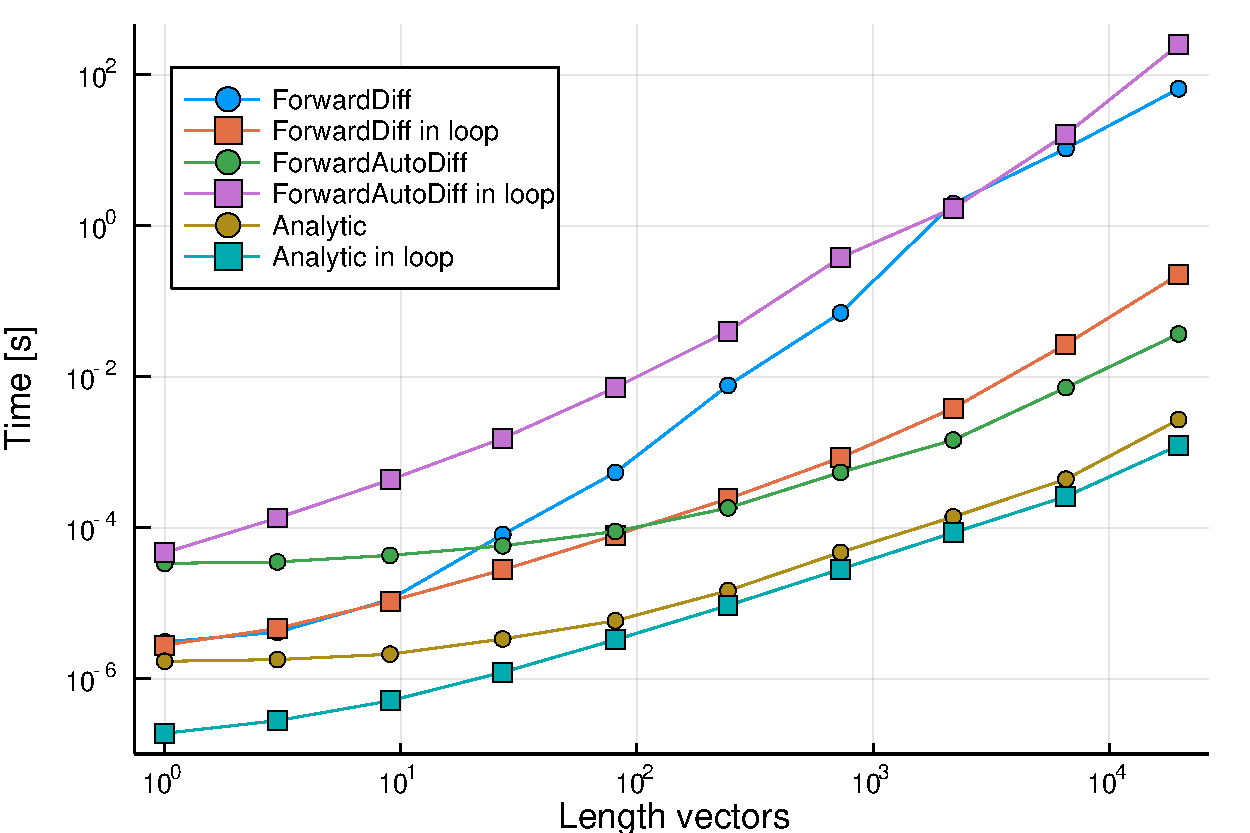
\includegraphics[width = 0.9\textwidth]{figures/benchmark_ad_in_loop.pdf}
    \caption{Computational time for calculating the value and gradient of $f$ in Equation \eqref{eq:benchmarkFunction} as                         a function of length of the input vectors.}
    \label{fig:benchmarkADInLoop}
\end{figure}

The first observation to make is that the \textit{ForwardAutoDiff} implementation is clearly not optimized for evaluating the vector function scalar by scalar, as it is the slowest method tested so far for all vector lengths. The next interesting observation is that Julia's implementation of AD, \textit{ForwardDiff}, can be made much more efficient in the evaluation of the vector function, by evaluating the function scalar by scalar. Using the method in \texttt{benchmarkADinLoop} with \textit{ForwardDiff}, we almost achieve the same test results as the regular \textit{ForwardAutoDiff} for long vectors. Although, it is important to mention that with the approach in \texttt{benchmarkADinLoop}, only the gradient of the function is obtained -- not the Jacobian. This limits the applicability of the method. In the particular case of the function $f$ in Equation \eqref{eq:benchmarkFunction}, the Jacobian will only be a diagonal matrix with the gradient of $f$ on the diagonal, but if we would evaluate a function like in Equation \eqref{eq:differenceFunction}, this approach would not work. Hence, although we almost manage to obtain the same performance in \textit{ForwardDiff} as we have in \textit{ForwardAutoDiff}, it comes with a cost that some types of functions cannot be evaluated. The implementation necessary to work around this and obtain the Jacobian with \textit{ForwardDiff} and \texttt{benchmarkADinLoop} will slow the computation down. For a vector function with large input vectors, \textit{ForwardAutoDiff} is therefore a better approach. 

Other than this, it is interesting to see that the evaluation of the analytical solution in a loop is faster than its vectorized counterpart. Here, Julia shows a real strength compared to MATLAB, where a function evaluation like the vector function $f$ will be much slower in a loop than with vector multiplication.
\begin{figure}[H]
    \centering
    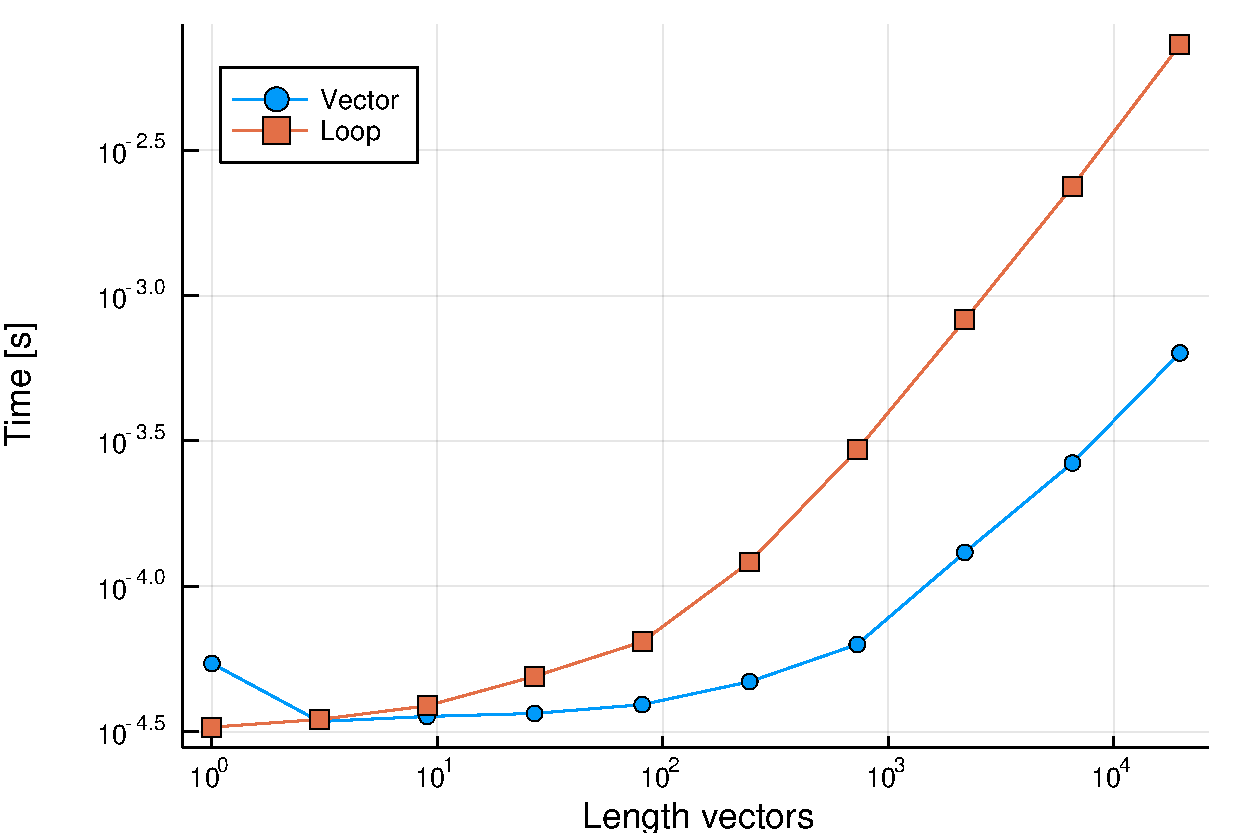
\includegraphics[width = 0.9\textwidth]{figures/benchmark_matlab_multiplication.pdf}
    \caption{Computational time for evaluating the analytic functions $f$, $f_x$, $f_y$ and $f_z$ from \eqref{eq:benchmarkFunction} as a function of length of the input vectors in MATLAB.}
    \label{fig:matlabMultiplication}
\end{figure}
\autoref{fig:matlabMultiplication} shows how much time MATLAB uses to evaluate the analytic functions $f$, $f_x$, $f_y$ and $f_z$ from Equation \eqref{eq:benchmarkFunction} as vector multiplication and in a for-loop. The analytic graphs in \autoref{fig:benchmarkADInLoop} demonstrates the time Julia uses to evaluate the same functions. Where the vector multiplication and for-loop scale equally good in Julia, and the for-loop actually perform better, MATLAB's for-loops scale much worse than the vector multiplication in contrast. This can be viewed as a first indication that the developers of Julia actually have managed to create a language with similar mathematical syntax as MATLAB and the computational efficiency of C.